\documentclass [12pt]{article}
\setlength{\parindent}{0em}
\setlength{\parskip}{0.25in}
\usepackage{geometry}
\geometry{verbose,letterpaper,tmargin=0.5in,bmargin=1.0in,lmargin=.70in,rmargin=.70in}
\usepackage{graphicx}
\usepackage{amsmath}
\usepackage{amssymb}
\usepackage{amsthm}
\theoremstyle{definition}
\newtheorem{exmp}{Example}[section]
\usepackage{tikz}
\usetikzlibrary{arrows,decorations.pathmorphing,backgrounds,positioning,fit,petri,calc,matrix}
\usepackage{slashbox}
\usepackage{listings}
\usepackage{ dsfont }
\usepackage{ upgreek }
\usepackage{graphicx}
\graphicspath{ {./images/} }


\newcommand{\ket}[1]{| {#1} \rangle}
\newcommand{\bra}[1]{\langle {#1} |}
\newcommand{\braket}[2]{\langle #1 \ | \ #2 \rangle}
\newcommand{\tensor}[2]{ #1 \otimes  #2 }

\definecolor{dkgreen}{rgb}{0,0.6,0}
\definecolor{gray}{rgb}{0.5,0.5,0.5}
\definecolor{mauve}{rgb}{0.58,0,0.82}

\lstset{frame=tb,
  language=Python,
  aboveskip=3mm,
  belowskip=3mm,
  showstringspaces=false,
  columns=flexible,
  basicstyle={\small\ttfamily},
  numbers=none,
  numberstyle=\tiny\color{gray},
  keywordstyle=\color{blue},
  commentstyle=\color{dkgreen},
  stringstyle=\color{mauve},
  breaklines=true,
  breakatwhitespace=true,
  tabsize=3
}

\DeclareMathOperator{\Cspan}{ \CC-span }

\title{Home Work 6}
\author{Madhu Peduri}
\date{03/13/2021}

\begin{document}
\section*{Homework 6}

{\bf 6.5.a.} Let $H = \dfrac{1}{\sqrt{2}}\begin{bmatrix} 1 & 1 \\ 1 & -1 \end{bmatrix}$. Write the matrix of the operator $H[2]$ acting on the space $B^{\otimes 3}$

\phantom{1em} {\bf 1.} We have qubit space of 3 and Hardman operator on subset of 2 qubits, given by below formula,\\
\phantom{1000em} $X[p] = I_{B^{\otimes (p-1)}} \otimes I_{B^{\otimes (n-p)}}$

\phantom{1em} {\bf 2.} In our case $n=3, p=2$, we get, $H[2] = I_{B^{\otimes (1)}} \otimes H \otimes I_{B^{\otimes (1)}}$\\\\
\phantom{1000em} $H[2] = \dfrac{1}{\sqrt{2}}\begin{bmatrix} 1 & 0 \\ 0 & 1 \end{bmatrix} \otimes \begin{bmatrix} 1 & 1 \\ 1 & -1 \end{bmatrix} \otimes \begin{bmatrix} 1 & 0 \\ 0 & 1 \end{bmatrix}$\\\\
\phantom{1000em} $= \dfrac{1}{\sqrt{2}}\begin{bmatrix} 1 & 1 & 0 & 0 \\ 1 & -1 & 0 & 0 \\ 0 & 0 & 1 & 1 \\ 0 & 0 & 1 & -1\end{bmatrix} \otimes \begin{bmatrix} 1 & 0 \\ 0 & 1 \end{bmatrix} = \dfrac{1}{\sqrt{2}}\begin{bmatrix} 1 & 0 & 1 & 0 & 0 & 0 & 0 & 0\\ 0 & 1 & 0 & 1 & 0 & 0 & 0 & 0\\1 & 0 & -1 & 0 & 0 & 0 & 0 & 0\\0 & 1 & 0 & -1 & 0 & 0 & 0 & 0\\0 & 0 & 0 & 0 & 1 & 0 & 1 & 0\\0 & 0 & 0 & 0 & 0 & 1 & 0 & 1\\0 & 0 & 0 & 0 & 1 & 0 & -1 & 0\\0 & 0 & 0 & 0 & 0 & 1 & 0 & -1\end{bmatrix}$

\newpage

{\bf 6.5.b.}\\
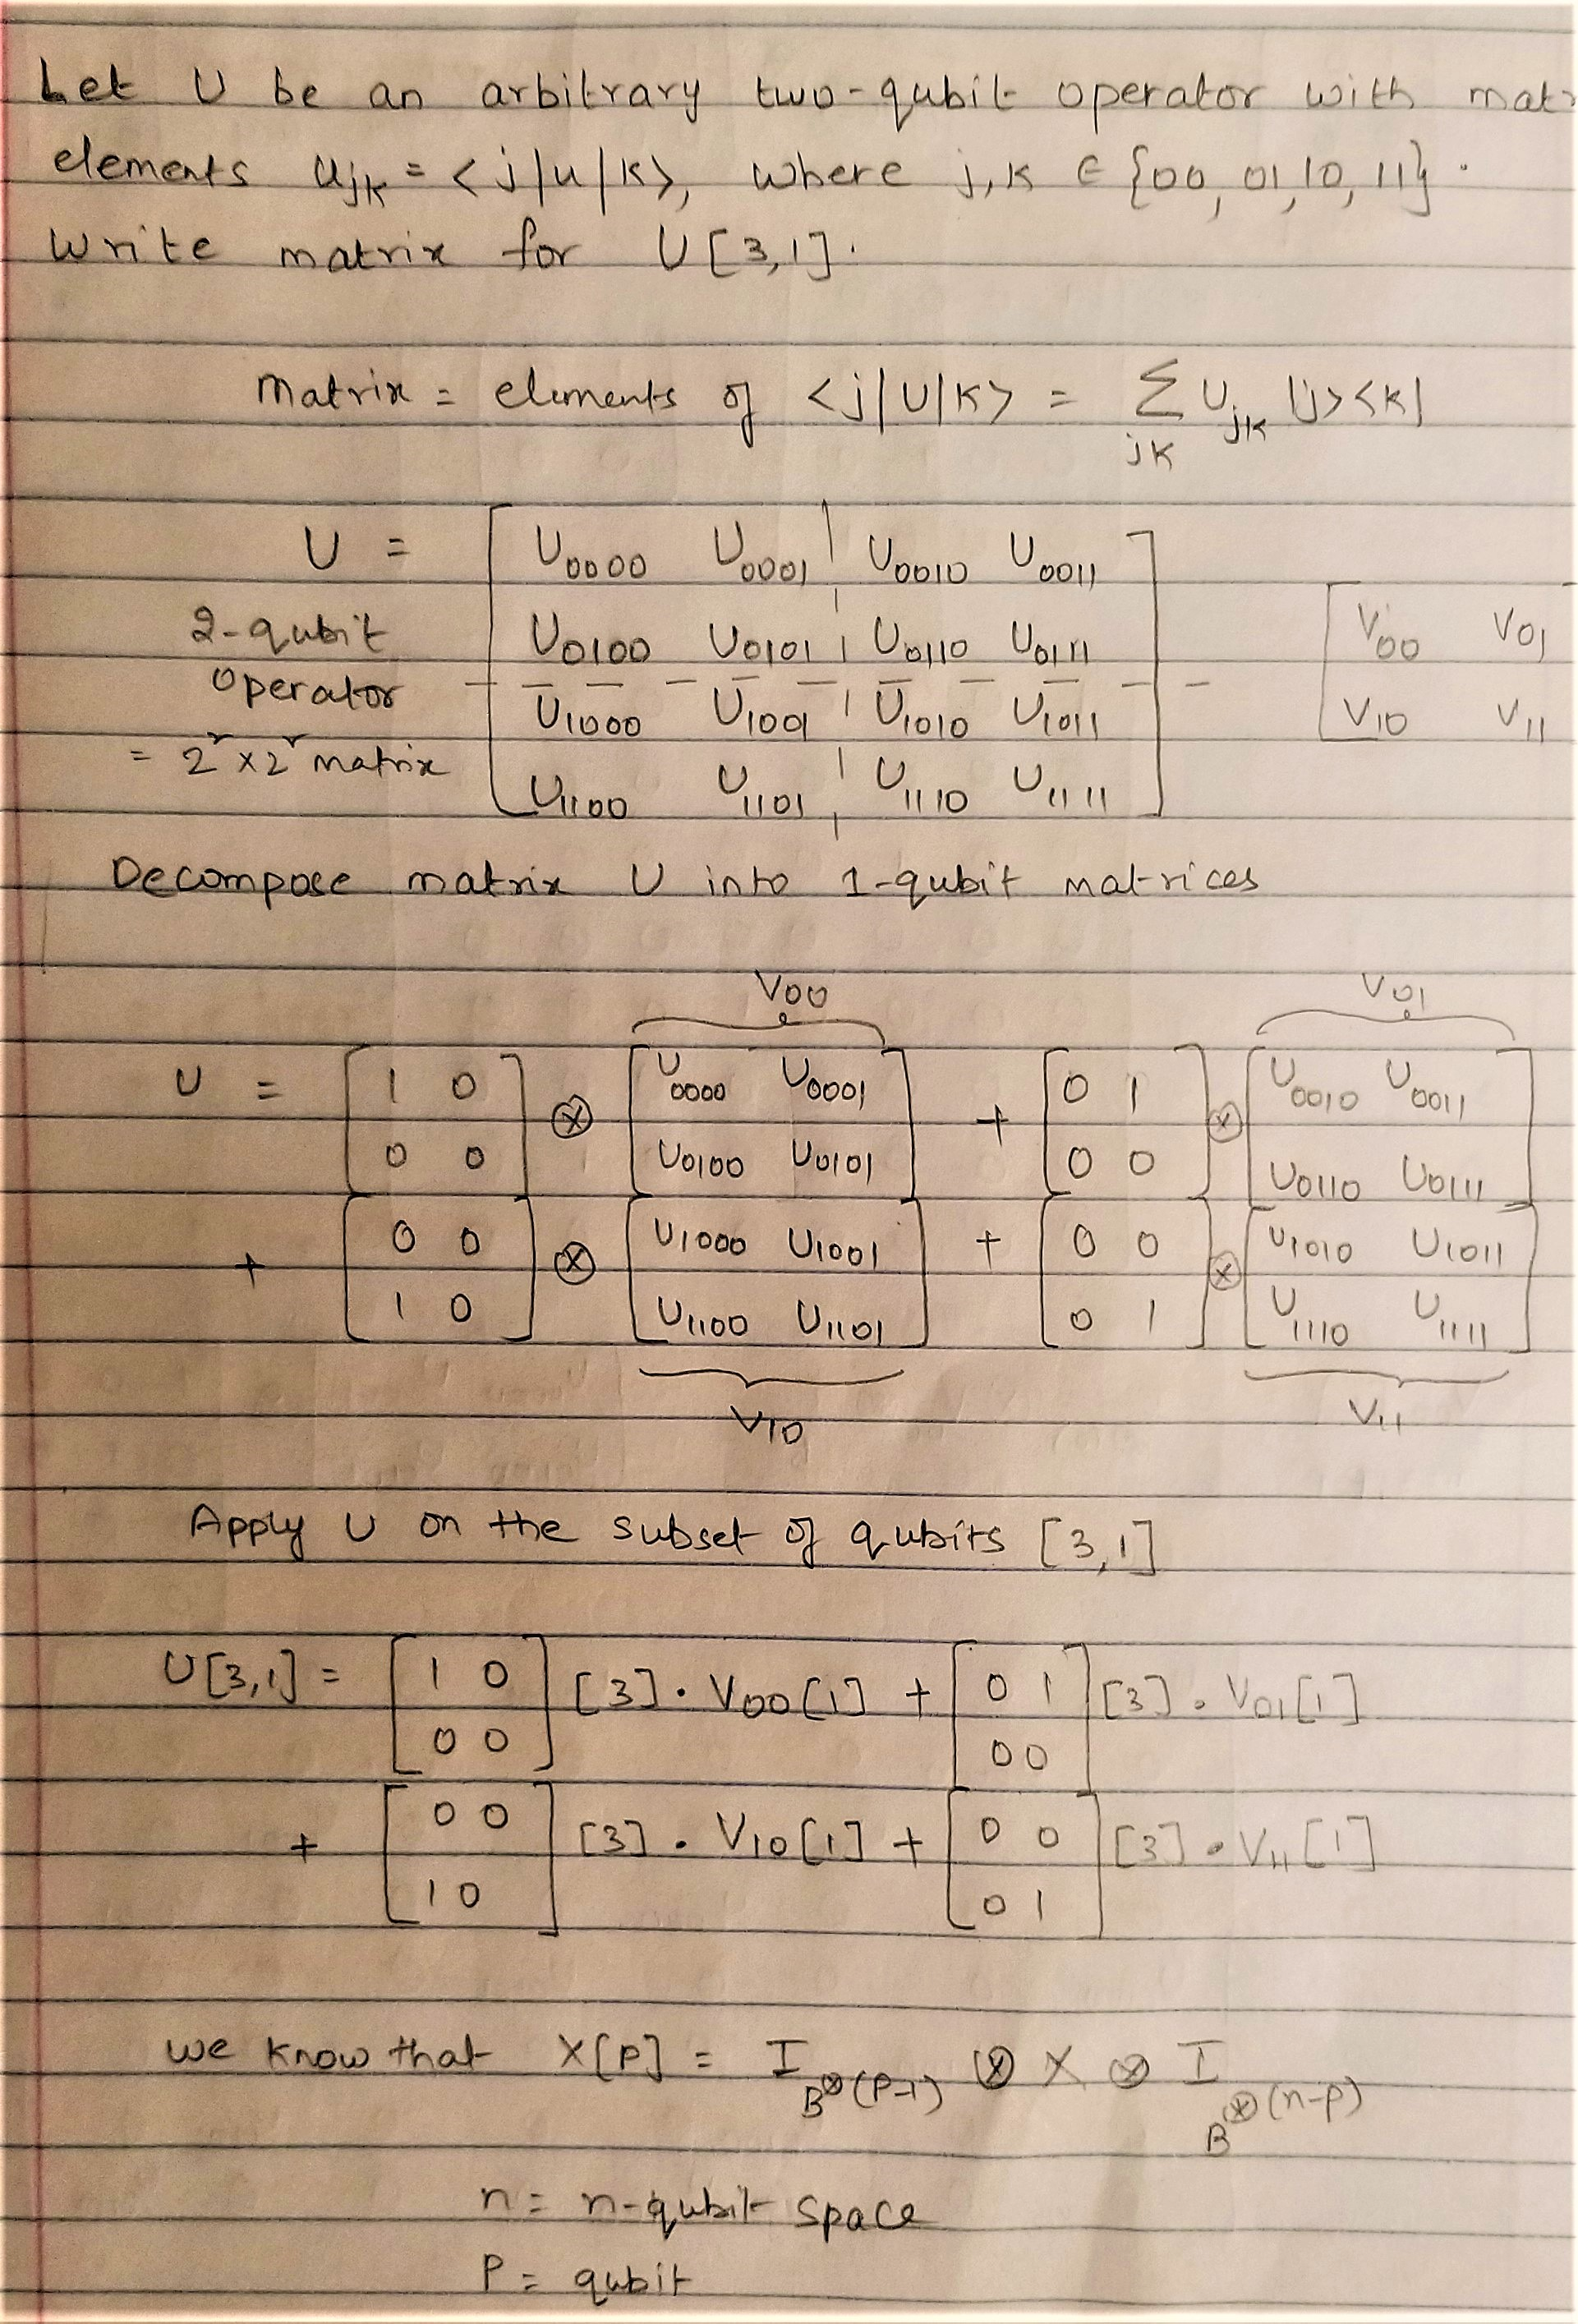
\includegraphics[width=18cm, height=23cm]{I11}\\
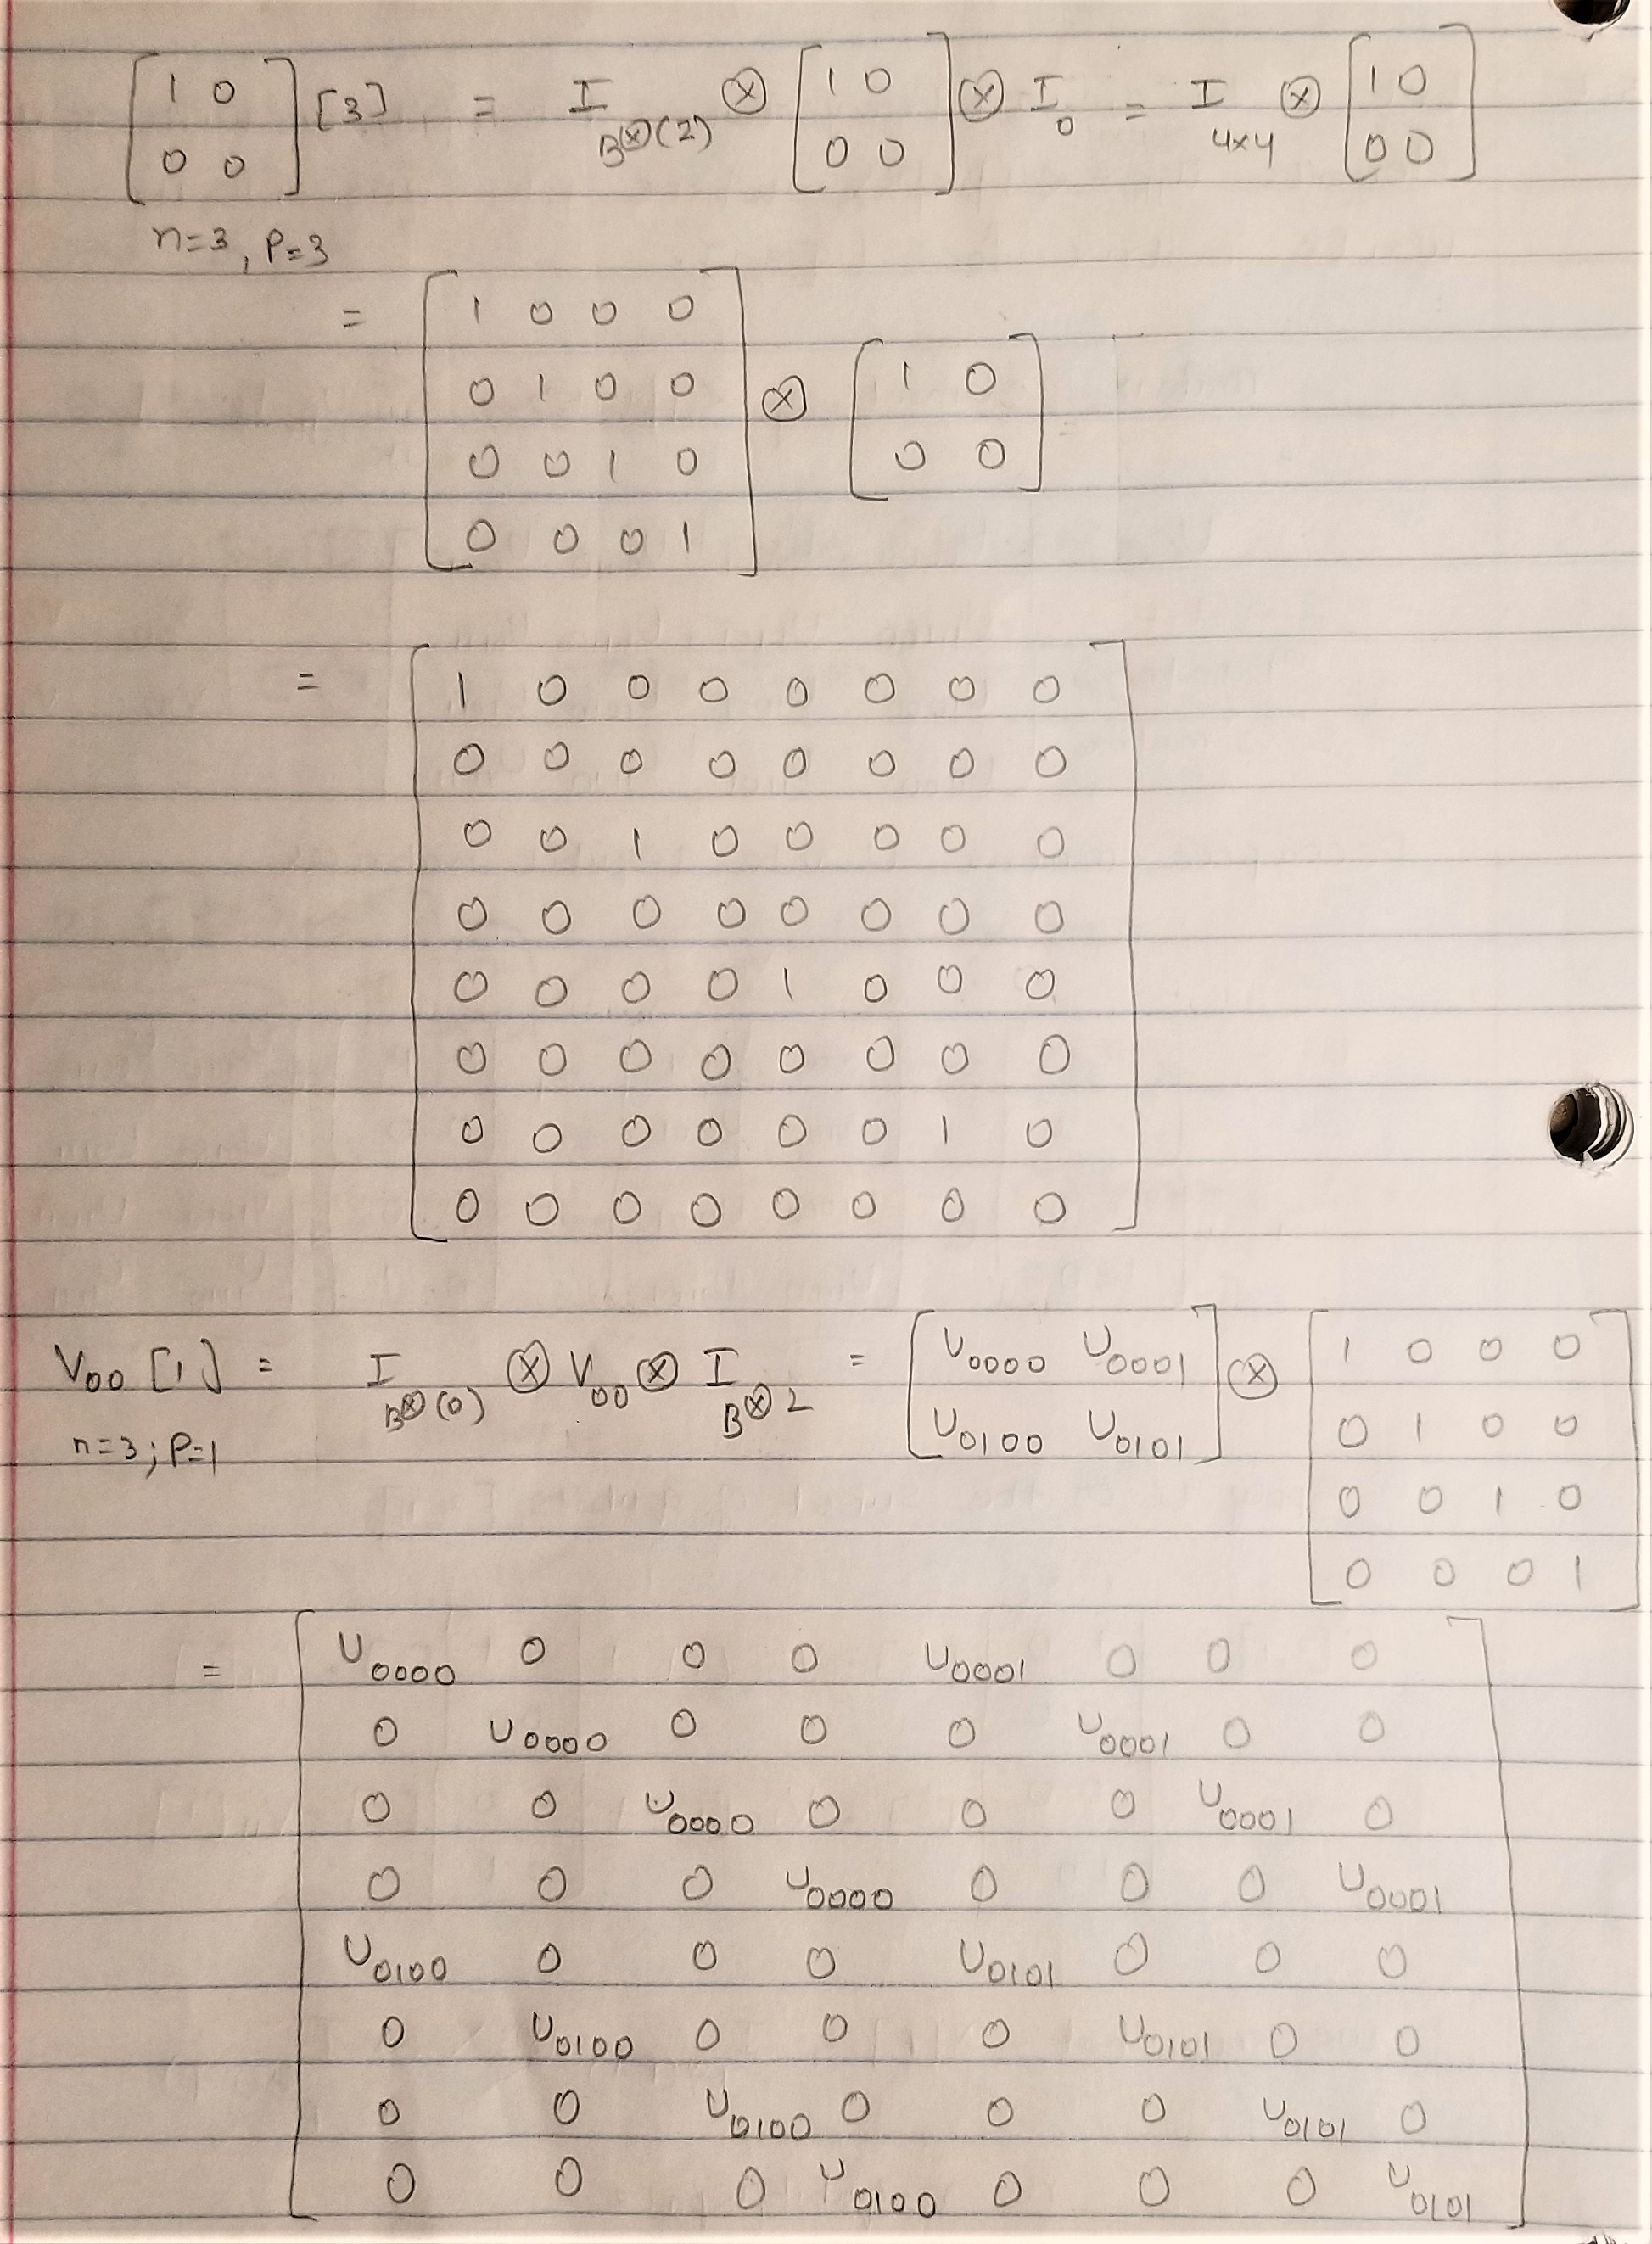
\includegraphics[width=18cm, height=23cm]{I22}\\
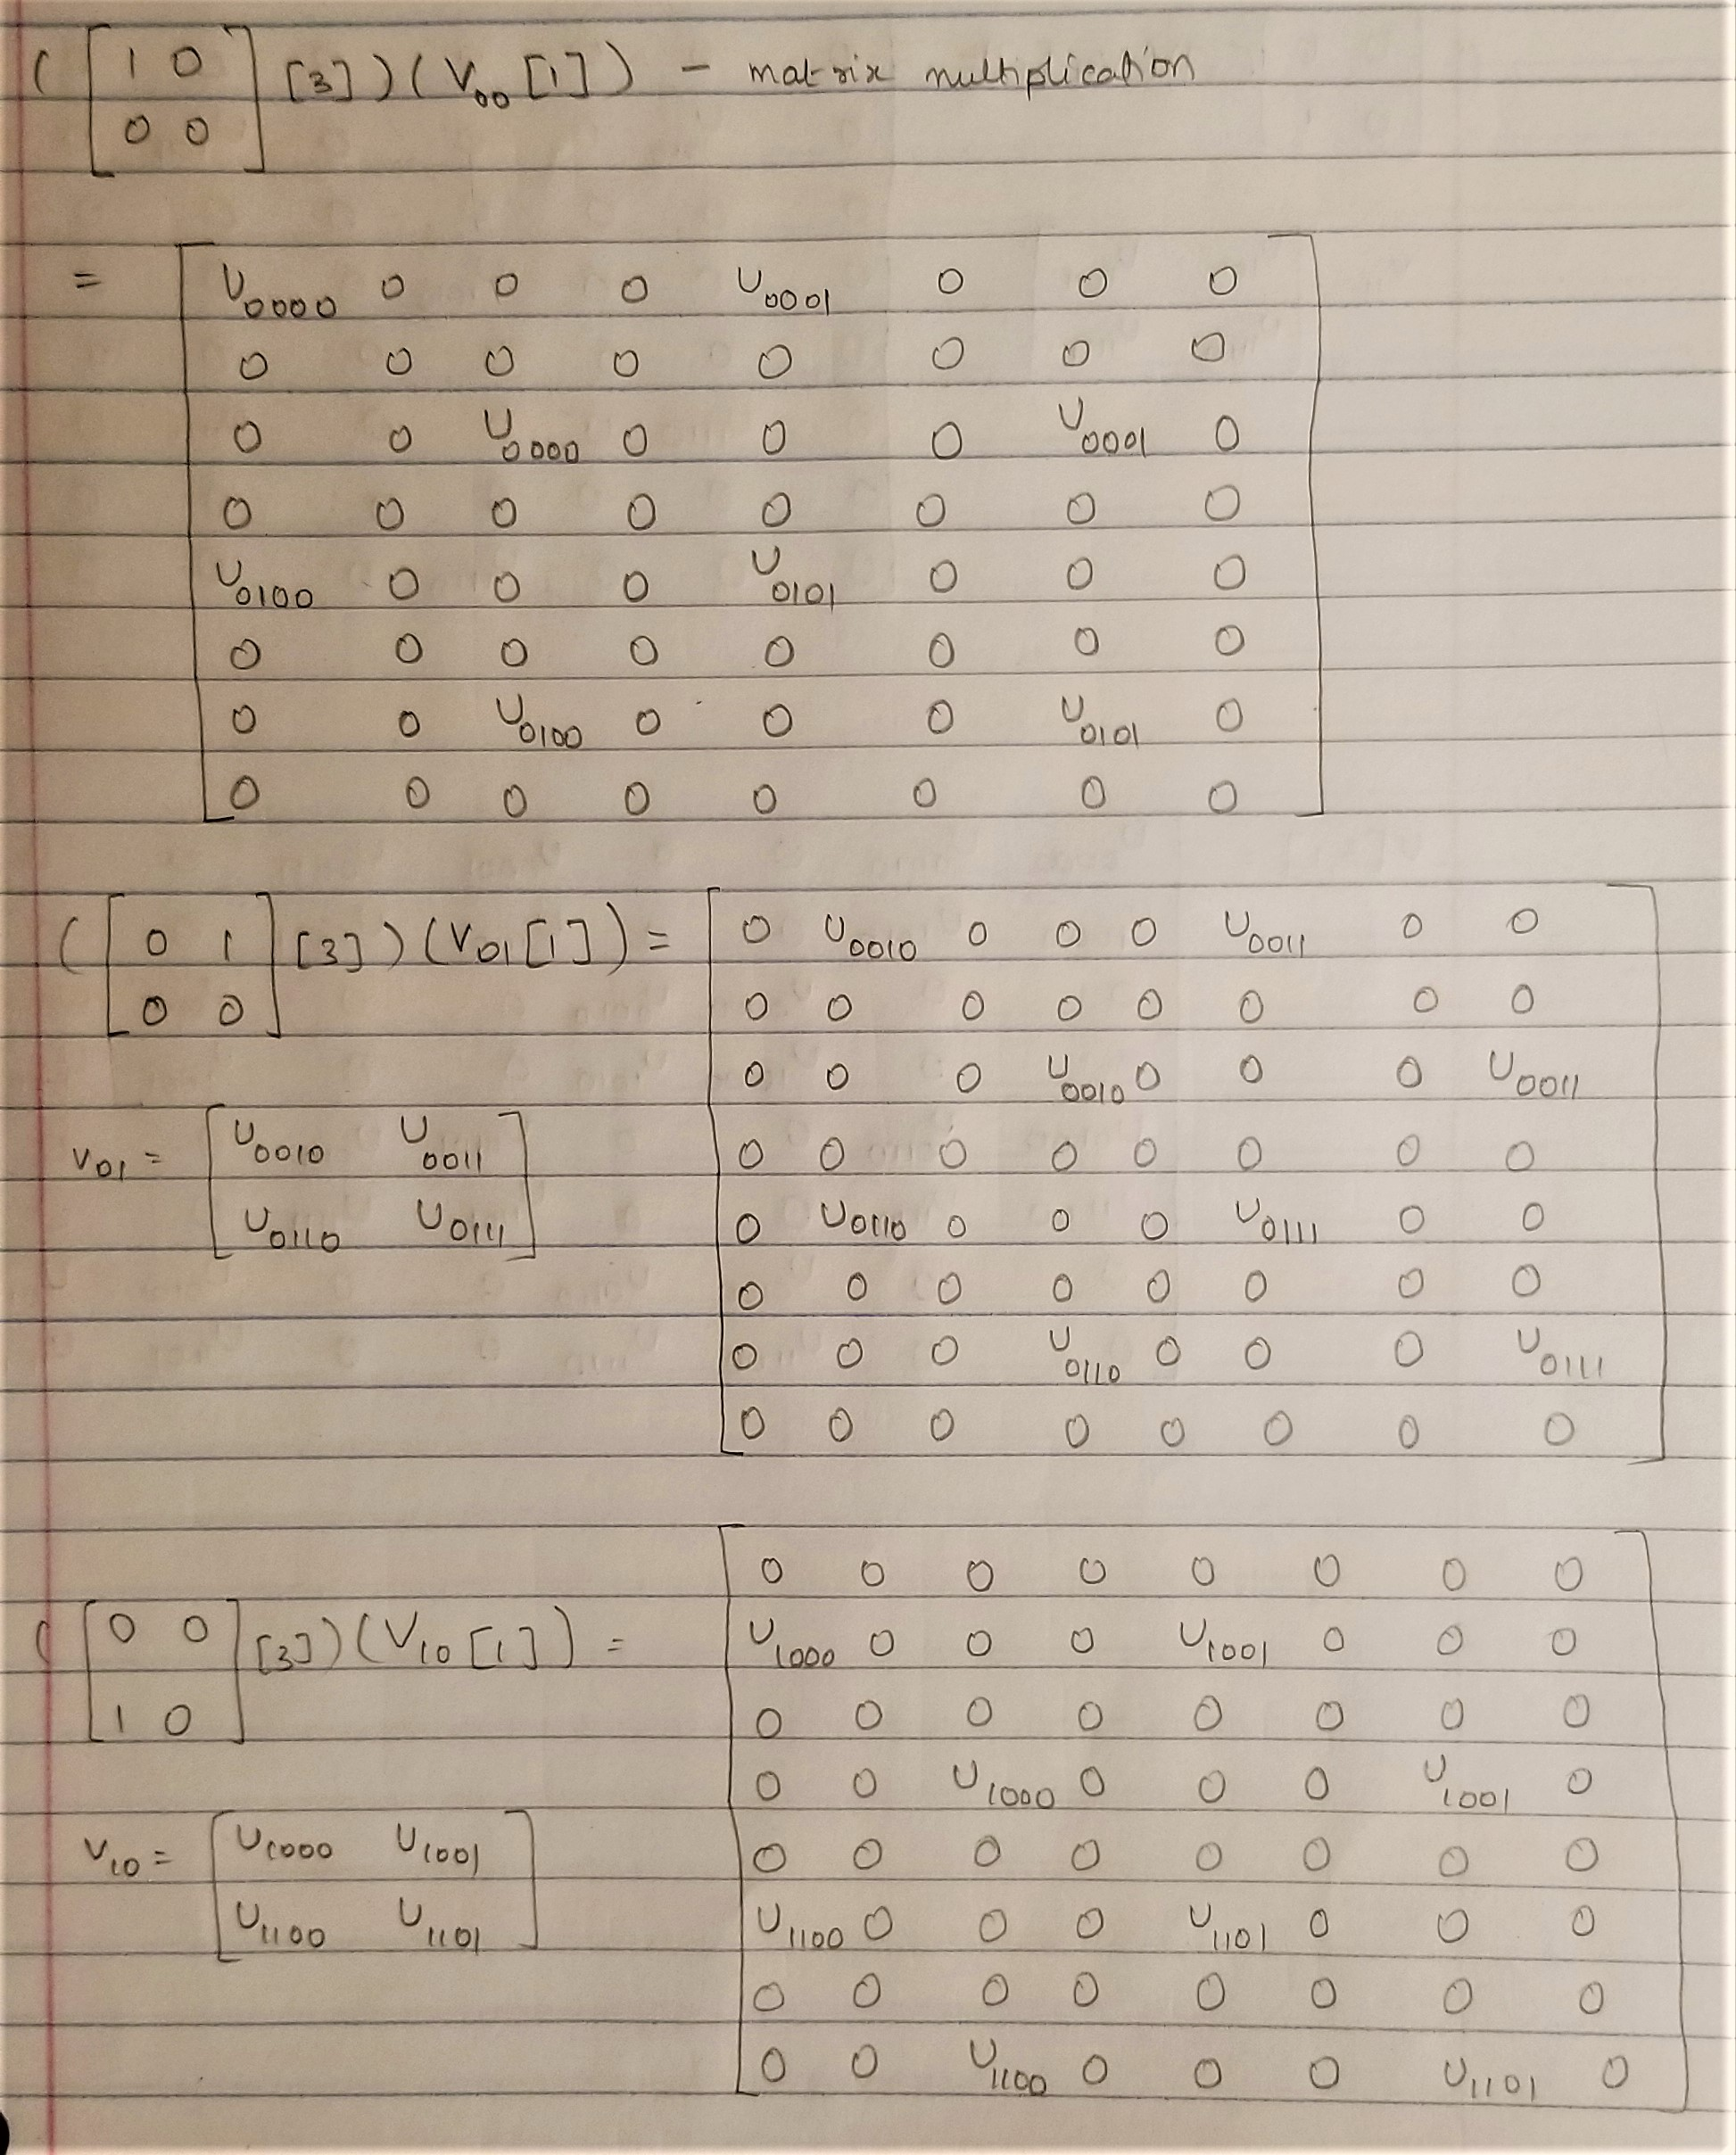
\includegraphics[width=18cm, height=23cm]{I33}\\
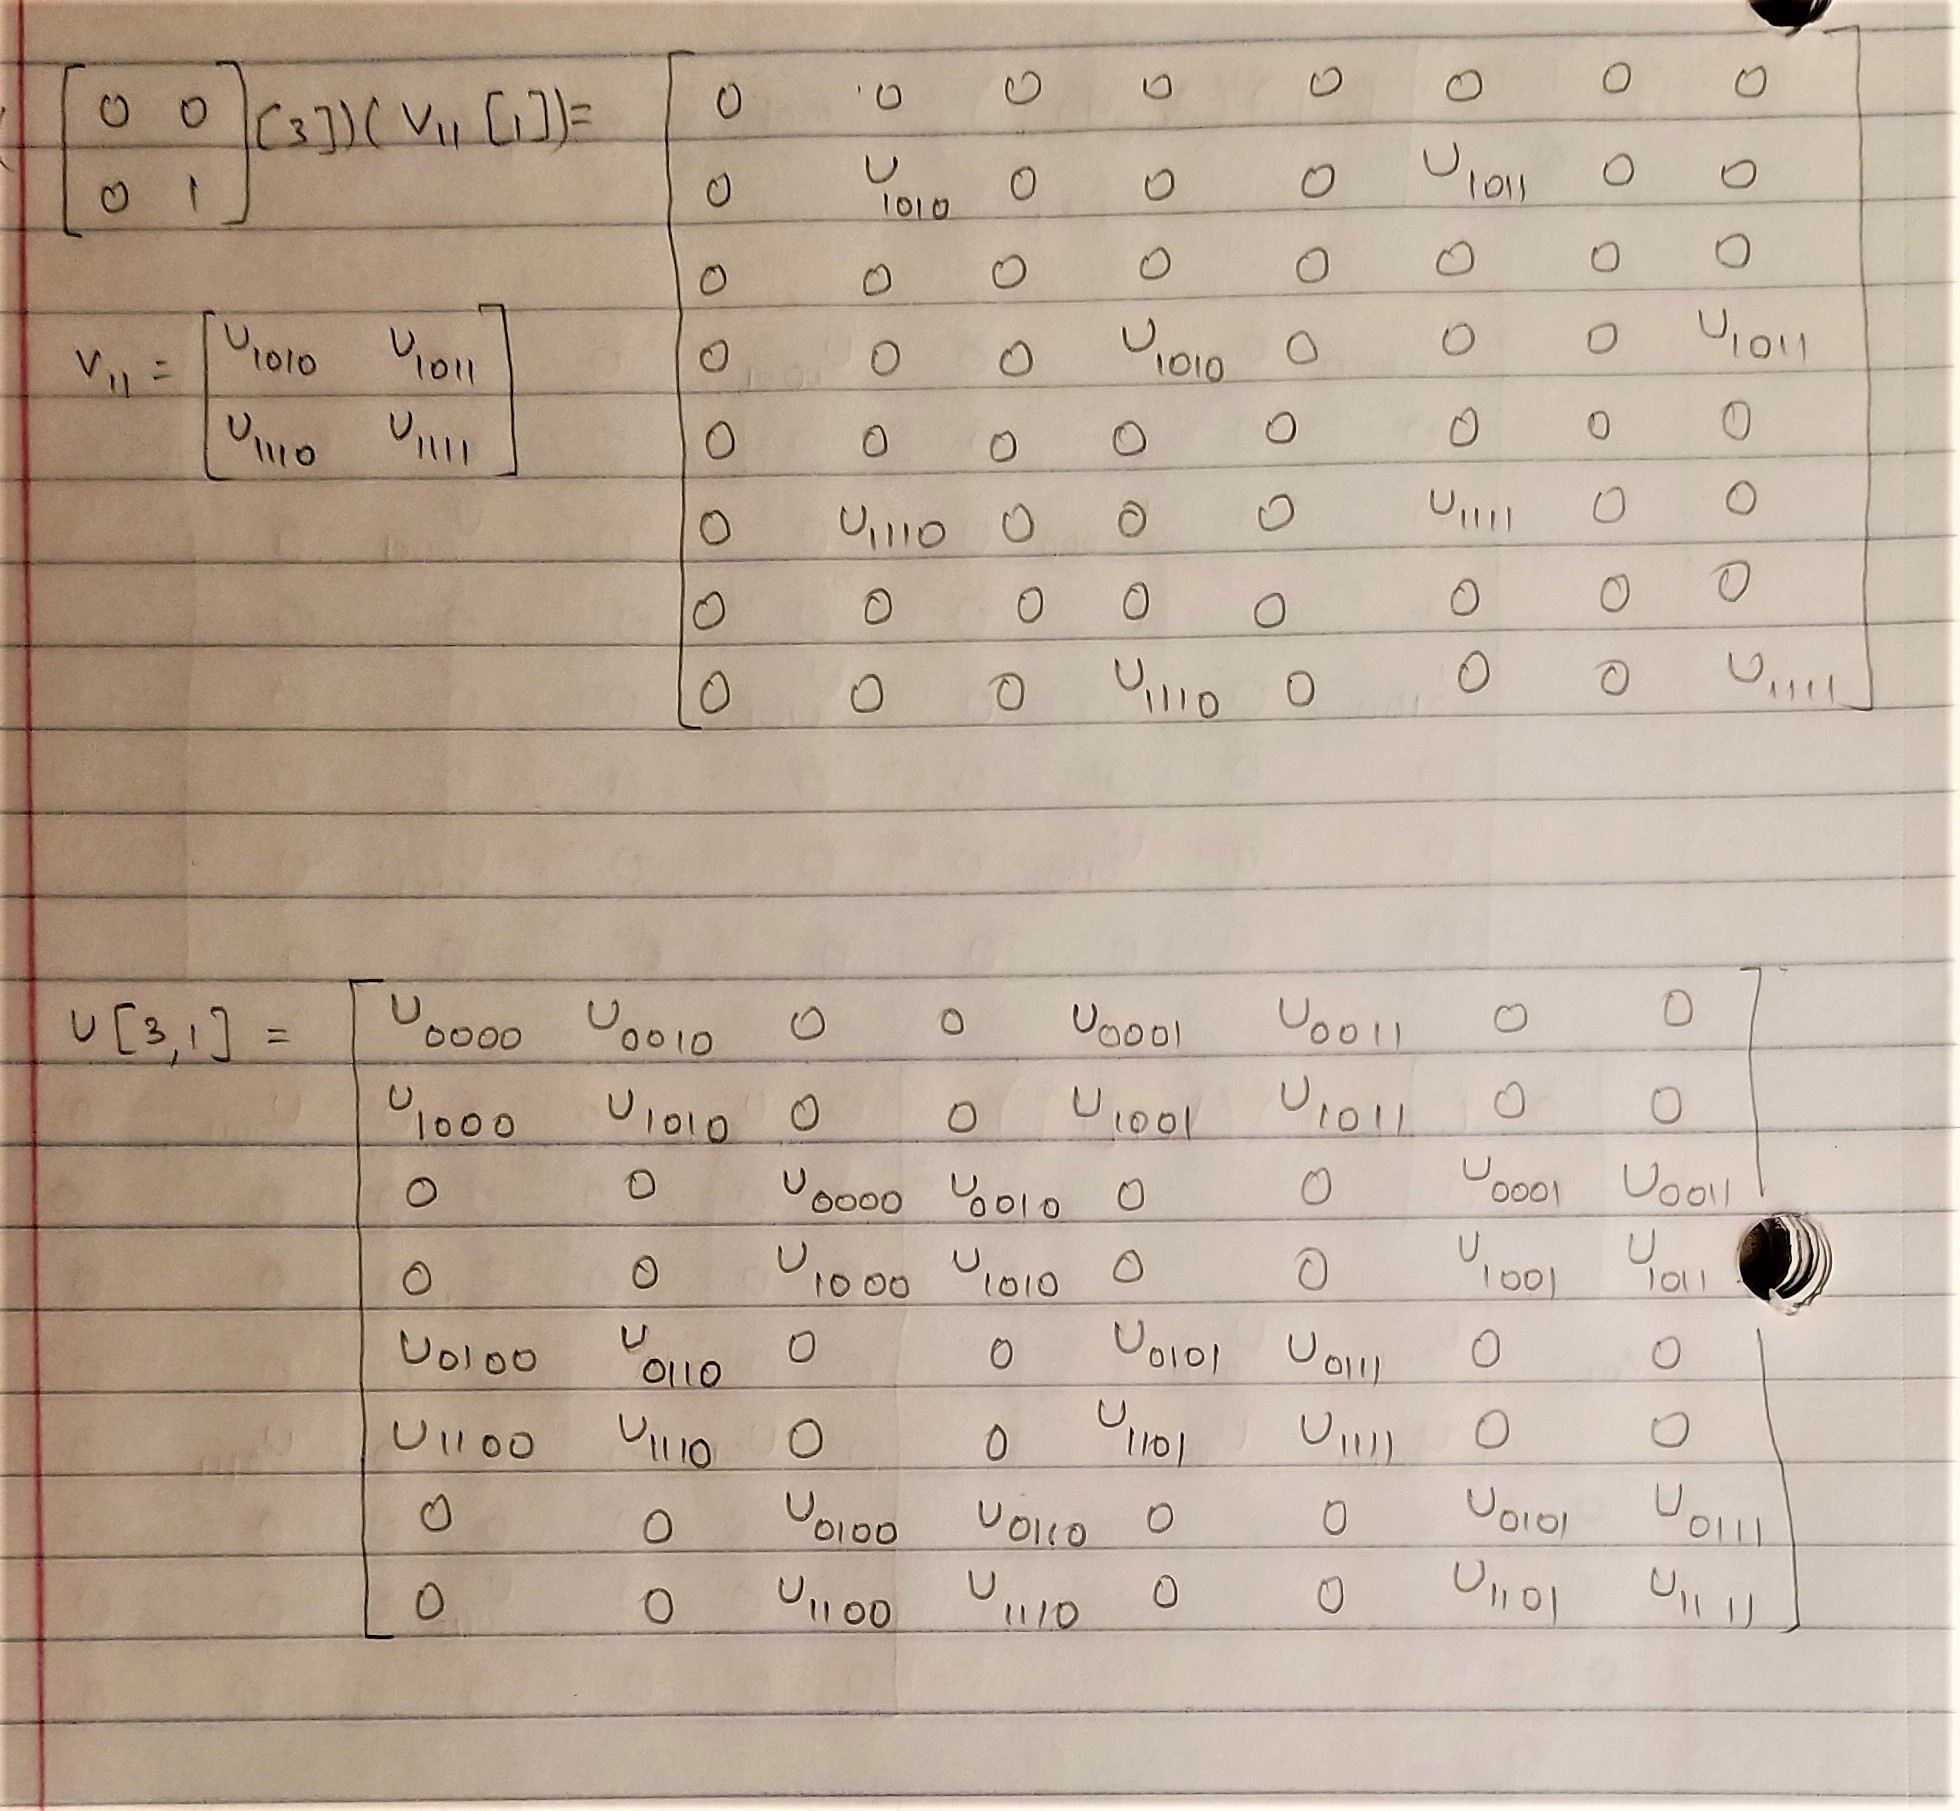
\includegraphics[width=18cm, height=23cm]{I44}

\newpage

{\bf 1.} Prove that the inner product and the tensor product commute: $\braket{\tensor{\alpha}{\beta}}{\tensor{\gamma}{\delta}} = \braket{\alpha}{\gamma} \braket{\beta}{\delta}$

\phantom{1em} {\bf 1.} We know that $\ket{\varepsilon} = \bra{\varepsilon^{\dag}}$, where $\dag = Conjugate \ transpose$. Let, 

\phantom{1000em} $\ket{\alpha} = \begin{bmatrix} \alpha_{1} \\ \alpha_{2}\end{bmatrix}, \ \ket{\beta} = \begin{bmatrix} \beta_{1} \\ \beta_{2}\end{bmatrix}, \ \ket{\gamma} = \begin{bmatrix} \gamma_{1} \\ \gamma_{2}\end{bmatrix}, \ \ket{\delta} = \begin{bmatrix} \delta_{1} \\ \delta_{2}\end{bmatrix}$

\phantom{1000em} $\bra{\alpha^{\dag}} = \begin{bmatrix} \alpha^{\dag}_{1} & \alpha^{\dag}_{2}\end{bmatrix}, \ \bra{\beta^{\dag}} = \begin{bmatrix} \beta^{\dag}_{1} & \beta^{\dag}_{2}\end{bmatrix}, \ \bra{\gamma^{\dag}} = \begin{bmatrix} \gamma^{\dag}_{1} & \gamma^{\dag}_{2}\end{bmatrix}, \ \bra{\delta^{\dag}} = \begin{bmatrix} \delta^{\dag}_{1} & \delta^{\dag}_{2}\end{bmatrix}$

\phantom{1em} {\bf 2.} Using above vectors, we can define tensors as below,

\phantom{1000em} $\ket{\tensor{\alpha}{\beta}} = \tensor{\begin{bmatrix} \alpha_{1} \\ \alpha_{2}\end{bmatrix}}{\begin{bmatrix} \beta_{1} \\ \beta_{2}\end{bmatrix}}$ and $\bra{\tensor{\alpha}{\beta}} = \tensor{\begin{bmatrix} \alpha^{\dag}_{1} & \alpha^{\dag}_{2}\end{bmatrix}}{\begin{bmatrix} \beta^{\dag}_{1} & \beta^{\dag}_{2}\end{bmatrix}} = \begin{bmatrix}\alpha^{\dag}_{1}\beta^{\dag}_{1} & \alpha^{\dag}_{1}\beta^{\dag}_{2} & \alpha^{\dag}_{2}\beta^{\dag}_{1} & \alpha^{\dag}_{2}\beta^{\dag}_{2}\end{bmatrix}$

\phantom{1000em} $\ket{\tensor{\gamma}{\delta}} = \tensor{\begin{bmatrix} \gamma_{1} \\ \gamma_{2}\end{bmatrix}}{\begin{bmatrix} \delta_{1} \\ \delta_{2}\end{bmatrix}} = \begin{bmatrix}\gamma_{1}\delta_{1} \\ \gamma_{1}\delta_{2} \\ \gamma_{2}\delta_{1} \\ \gamma_{2}\delta_{2}\end{bmatrix}$

\phantom{1000em} $\braket{\tensor{\alpha}{\beta}}{\tensor{\gamma}{\delta}} = \alpha^{\dag}_{1}\beta^{\dag}_{1}\gamma_{1}\delta_{1} + \alpha^{\dag}_{1}\beta^{\dag}_{2}\gamma_{1}\delta_{2} + \alpha^{\dag}_{2}\beta^{\dag}_{1}\gamma_{2}\delta_{1} + \alpha^{\dag}_{2}\beta^{\dag}_{2}\gamma_{2}\delta_{2}$

\phantom{1em} {\bf 3.} We will derive inner product as below,

\phantom{1000em} $\braket{\alpha}{\gamma} = \begin{bmatrix} \alpha^{\dag}_{1} & \alpha^{\dag}_{2}\end{bmatrix}\begin{bmatrix} \gamma_{1} \\ \gamma_{2}\end{bmatrix} = \alpha^{\dag}_{1}\gamma_{1} + \alpha^{\dag}_{2}\gamma_{2}$ and $\braket{\beta}{\delta} = \begin{bmatrix} \beta^{\dag}_{1} & \beta^{\dag}_{2}\end{bmatrix}\begin{bmatrix} \delta_{1} \\ \delta_{2}\end{bmatrix} = \beta^{\dag}_{1}\delta_{1} + \beta^{\dag}_{2}\delta_{2}$

\phantom{1000em} $\braket{\alpha}{\gamma} \braket{\beta}{\delta} = [\alpha^{\dag}_{1}\gamma_{1} + \alpha^{\dag}_{2}\gamma_{2}][\beta^{\dag}_{1}\delta_{1} + \beta^{\dag}_{2}\delta_{2}] = \alpha^{\dag}_{1}\beta^{\dag}_{1}\gamma_{1}\delta_{1} + \alpha^{\dag}_{1}\beta^{\dag}_{2}\gamma_{1}\delta_{2} + \alpha^{\dag}_{2}\beta^{\dag}_{1}\gamma_{2}\delta_{1} + \alpha^{\dag}_{2}\beta^{\dag}_{2}\gamma_{2}\delta_{2}$

\phantom{1em} {\bf 4.} From the results of point 2 and 3, we can say that,

\phantom{1000em} $\braket{\tensor{\alpha}{\beta}}{\tensor{\gamma}{\delta}} = \braket{\alpha}{\gamma} \braket{\beta}{\delta}$\\

\newpage

{\bf 2.} An $n-ary$ function 

\end{document}